%        File: Report.tux
%     Created: 二 11月 28 03:00 下午 2017 C
% Last Change: 二 11月 28 03:00 下午 2017 C
%
\documentclass[UTF8,noindent]{ctexart}
\usepackage[a4paper,left=2.0cm,right=2.0cm,top=2.0cm,bottom=2.0cm]{geometry}
\usepackage{graphicx}
\usepackage{amsmath}
\usepackage{amssymb}
\usepackage{xeCJK}
\usepackage{listings}
\usepackage{float}
\CTEXsetup[format={\Large\bfseries}]{section}

\title{Project4\ Synchronization\ Primitives\ and\ IPC\ 设计文档}

\author{冯吕\ $2015K8009929049$}
\date{\today}
\begin{document}
\maketitle
\zihao{5}
\CJKfamily{zhsong}

\section*{一、do\_spawn, do\_wait 和 do\_kill 的设计}

\subsection*{1.do\_spawn 的处理过程}
do\_spawn()函数是一个系统调用,它需要根据提供的的参数(任务名字),在Files.c文件中找到对应的任务信息,根据这些信息,对任务进行初始化,首先,初始化$PCB$,然后将任务加入到就绪队列中。

当任务名字传入do\_spawn()函数之后,它首先调用ramdisk\_find\_File()函数找出任务对应的信息:即任务的入口地址和任务类型,之后,对$PCB$进行初始化,然后再将初始化后的$PCB$加入到就绪队列中。

由于$PCB$本身是一个数组,因此,初始化$PCB$的时候首先找到一个未被使用的$PCB$项,即对应状态为$EXITED$,将该项的$index$作为新创建任务的$PID$,由于每一个$index$都是唯一的,因此$PID$也是唯一的。

\subsection*{2.do\_kill 的处理过程}

do\_kill()系统调用接受一个参数:$PID$。当进入处理过程之后,由于$PID$就等于$PCB$的$index$,因此,可直接获取需要kill的进程的$PCB$信息。

首先,用一个变量将该任务的状态保存下来,然后将$PCB$中其状态置为$EXITED$,即将该$PCB$资源回收。

另外,对于栈的回收,由于初始化$PCB$的函数是一直往下分配栈,所以如果不修改该函数的话,是无法对栈进行回收的。

之后,根据该进程被$kill$时候的状态,若为$ready$,则到$ready$对列中,找到对应的任务,将其$remove$;若为$BLOCKED$或$SLEEPING$,则到$wait$队列中,找到对应的任务,将其$remove$。

\subsection*{3.do\_wait 的处理过程}
当一个$task$调用do\_wait()系统调用时,需要等某一个特定任务退出或被$kill$,才能继续执行。

do\_wait()传入的参数为需要等待的任务$PID$,根据该$PID$,找出对应的任务,查看该任务的状态,若该任务的状态为$EXITED$,则退出,否则,do\_yiled(),等到再次回来时,再查看需要等待的任务是否已经退出,不退出则继续do\_yiled()。

\begin{figure}[H]
  \centering
  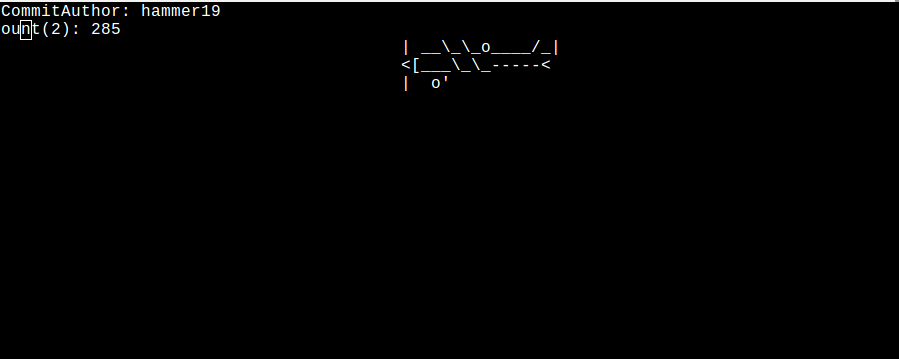
\includegraphics[scale=0.3]{spwan.png}
  \caption{do\_spwan()测试}
\end{figure}

\section*{二、同步原语设计}
\subsection*{1.条件变量}
条件变量是管程内的等待机制,每个条件变量表示一种等待原因和对应一个等待队列。如果条件不被满足,则进程被阻塞,即Wait()操作,直到被唤醒(Signal()或Broadcast()操作)。另外,条件变量还需要结合锁来实现。

在本次实验中,定义的条件变量的结构如下:
\begin{lstlisting}[language=c]
typedef struct condition{
	int wait_num;
	node_t cond_wait_queue;

} condition_t;
\end{lstlisting}
该结构包含两个成员,一个$wait\_num$表示目前阻塞的任务数量,另一个为阻塞队列。

条件变量有四个操作:初始化,Wait() 和 Signal() 和 Broadcast()。其实现均非常简单,初始化时只需要将 Wait\_num 初始化为0,同时将初始化等待队列即可;Wait()操作则将当前任务阻塞;Signal()操作唤醒一个阻塞的任务,如果没有任务被阻塞,则等同于空操作;Broadcast()则唤醒所有被阻塞的任务。
\subsection*{2.信号量}
信号量是操作系统提供的一种协调共享资源访问的方法。它由三个部分组成,一个整形变量,表示系统资源的数量,以及两个原子操作,P()操作或down()操作需要等待信号量为正,并将其减一,V()操作或up()操作则将信号量加一。

在本次实验中,信号量的结构定义如下:
\begin{lstlisting}[language=c]
typedef struct semaphore{
	int sem;
	node_t sem_wait_queue;

} semaphore_t;
\end{lstlisting}
一个整形变量表示信号量的数量,另一个为等待队列。

\subsection*{3.屏障}
屏障是指多个进程或线程,所有进程或线程都要到达某一个点之后,才能够往后执行,只要有一个没有到达,那么其他进程就需要等待,因此,就相当于一个屏障。

在本次实验中,屏障的结构定义如下:
\begin{lstlisting}[language = c]
typedef struct barrier{
	int wait_task_num;
	int all_task_num;
	node_t barrier_wait_queue;

} barrier_t;
\end{lstlisting}
$wait\_task\_num$ 表示当前已经处于等待中的任务数量,$all\_task\_num$表示所有任务数量。初始化时,对等待队列进行初始化,同时将$all\_task\_num$ 设定为指定的值。它对应的操作只有一个:barrierWait(),到该函数以后,首先将$wait\_task\_num$加一,如果还小于$all\_task\_num$则,阻塞,否则,唤醒所有阻塞的任务。

\begin{figure}[H]
  \centering
  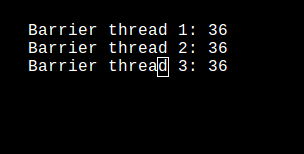
\includegraphics[height = 5cm ,width = 12cm]{barrier.png}
  \caption{test\_barrier测试}
\end{figure}

\begin{figure}[H]
  \centering
  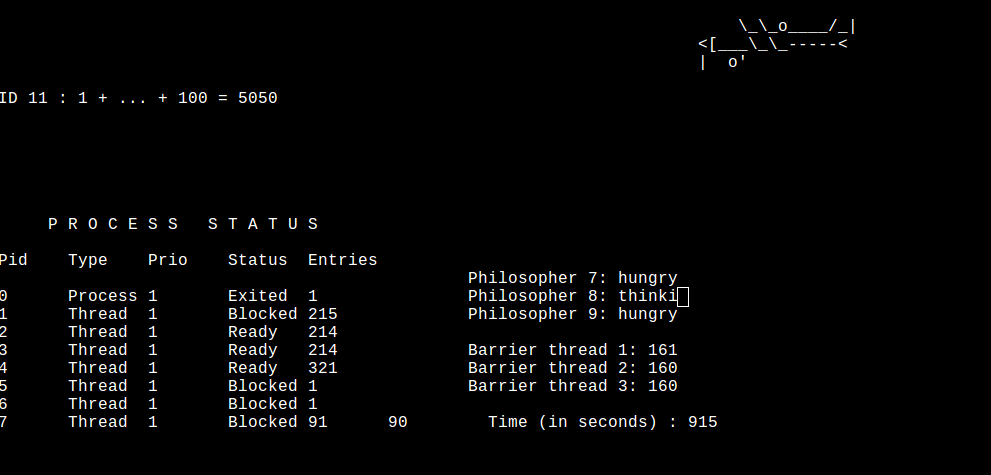
\includegraphics[height = 5cm, width = 12cm]{all.png}
  \caption{test\_all测试}
\end{figure}

\section*{三、mailbox设计}
\subsection*{1.$mailbox$数据结构}
在本次实验中,我的$mailbox$的结构定义如下:
\begin{lstlisting}[language=c]
typedef struct
{
	char name[MBOX_NAME_LENGTH];
	char buf[MAX_MBOX_LENGTH];
	int next_buf;
	condition_t Buf_full, Buf_empty;
	int turn;
	lock_t BoxLock;
} MessageBox;
\end{lstlisting}
$name$为$mailbox$的名字,$buf$用来存放$message$,$next\_buf$是$buf$中下一个可以存放的位置的$index$,两个条件变量$Buf\_full$和$Buf\_empty$表示$buf$满还是空,最后是$mailbox$的锁。

由于$buf$相当于一个静态对列,为了防止假满,每次从$buf$中读出数据之后,都把后面的数据往前面移动,相当于队列的$head$固定为了$0$,因此,只需要用一个$next_buf$来表明$buf$的情况,$next_buf$就相当于队尾。

\subsection*{2.生产者-消费者问题及$mailbox$实现}

生产者消费者问题是一个多线程同步的问题,在该问题中,两个线程共享一个有限大小的缓冲区,生产者将数据放到缓冲区,消费者从缓冲区中取数据,因此,需要保证,当缓冲区满了以后,生产者不能继续往里面放数据;当缓冲区空了以后,则消费者不能往里面取东西。

本次实验的$mailbox$问题就是一个生产者消费者的问题:$mailbox$的大小是有限的,只能放$MAX\_MBOX\_LENGTH$个字节,同时发送方相当于一个生产者,而接收方就相当于一个消费者。

使用条件变量即可解决该问题,$Buf\_full$表示缓冲区已经满,此时发送方便会被阻塞,直到被唤醒,而$Buf\_empty$则会把接收方阻塞。同时,每次只能有一个线程访问缓冲区,因此还要使用一个锁来实现缓冲区的互斥访问。

\begin{figure}[H]
  \centering
  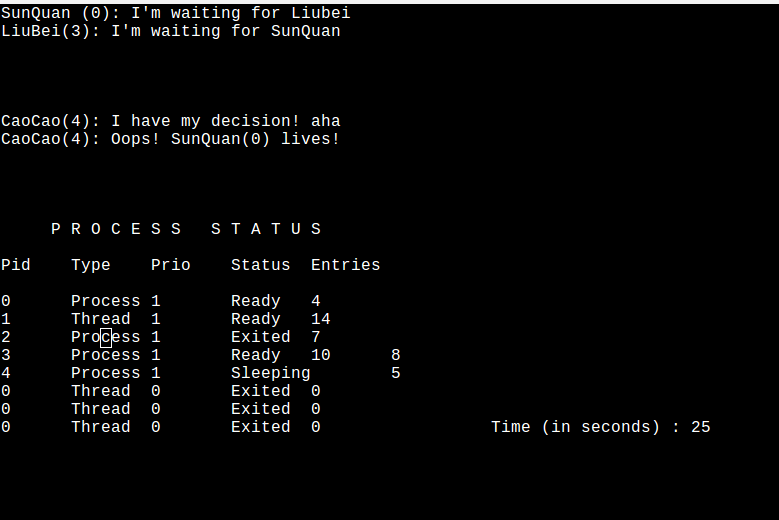
\includegraphics[scale = 0.5]{sanguo.png}
  \caption{test\_sanguo测试}
\end{figure}
\section*{四、关键函数功能}
1.do\_spawn()函数
\begin{lstlisting}[language =c]
static int do_spawn(const char *filename)
{
  (void)filename;
  int i;

  File *proc_file; //find process
  proc_file = ramdisk_find_File( filename );
  if ( !proc_file )
	return 0;

  struct task_info new_task; //task_info
  new_task.entry_point = proc_file->process;
  new_task.task_type = proc_file->task_type;

  for ( i = 0; i < NUM_PCBS; i++ ) //find empty pcb
	if (pcb[i].status == EXITED)
	  break;
  initialize_pcb( &pcb[i], i, &new_task ); //initial pcb and create process
  enqueue( &ready_queue, (node_t *)&(pcb[i]) ); 
  spawn_times++;
  return 0;
}
\end{lstlisting}
该函数根据提供的$task$的名字在$files.c$中找到对应的任务信息,并将其初始化,然后加入到$ready$队列中。

2.do\_kill()函数
\begin{lstlisting}[language=c]
static int do_kill(pid_t pid)
{
  enter_critical();
  pcb[pid].status = EXITED;
  pcb[pid].node.prev->next = pcb[pid].node.next;
  pcb[pid].node.next->prev = pcb[pid].node.prev;
\end{lstlisting}
该函数将$pid$指定的任务$kill$并回收$PCB$,将其从队列中移除。


3.condition\_wait()函数
\begin{lstlisting}[language=c]
void condition_wait(lock_t * m, condition_t * c){
	lock_release(m);
	enter_critical();
	c->wait_num++;
	block(&(c->cond_wait_queue));
	leave_critical();
	lock_acquire(m);
}
\end{lstlisting}
该函数释放所,然后将自己阻塞,等到再次回来之后立刻获得锁。

4.condition\_signal()函数
\begin{lstlisting}[language=c]
void condition_signal(condition_t * c){
	enter_critical();
	if (!c->wait_num)
	  ;
	else{
		unblock_one( &(c->cond_wait_queue) );
	}
	  leave_critical();
}
\end{lstlisting}
该函数从条件变量对应的等待队列中唤醒一个任务,如果等待队列中没有任务被阻塞,则等同于空操作。


5.condition\_broadcast()函数
\begin{lstlisting}[language=c]
void condition_broadcast(condition_t * c){
	enter_critical();
	while (c->wait_num--){
		unblock_one( &(c->cond_wait_queue) );
	}
	leave_critical();
}
\end{lstlisting}
该函数将条件变量中的所有被阻塞的任务唤醒,如果没有任务被阻塞,则等同于空操作。

6.semaphore\_up()函数
\begin{lstlisting}[language=c]
void semaphore_up(semaphore_t * s){
	enter_critical();
	s->sem++;
	if (s->sem >= 0)
	  unblock_one(&(s->sem_wait_queue));
	leave_critical();
}
\end{lstlisting}
该函数将信号量加一,如果之后信号量大于等于$0$,则唤醒一个阻塞任务。

7.semaphore\_down()函数
\begin{lstlisting}[language=c]
void semaphore_down(semaphore_t * s){
	enter_critical();
	s->sem--;
	if (s->sem < 0){
		block(&(s->sem_wait_queue));
	}
	leave_critical();
}
\end{lstlisting}
该函数将信号量减一,如果之后信号量小于$0$,则阻塞。

8.barrier\_wait()函数
\begin{lstlisting}[language=c]
void barrier_wait(barrier_t * b){
	enter_critical();
	b->wait_task_num++;
	if (b->wait_task_num < b->all_task_num){
		block(&(b->barrier_wait_queue));
	}
	else{
		while ( unblock_one(&(b->barrier_wait_queue)))
		  ;
		b->wait_task_num = 0;
	}
	leave_critical();
}
\end{lstlisting}
该函数首先将等待进程数量加一,如果还小于总的数量,则阻塞,否则,唤醒阻塞队列中的所有任务。

9.init\_mbox()函数
\begin{lstlisting}[language=c]
void init_mbox(void)
{
	int i;
	for ( i = 0; i < MAX_MBOXEN; i++ ){
		enter_critical();
		MessageBoxen[i].name[0] = '\0';
		MessageBoxen[i].next_buf = 0;
		MessageBoxen[i].turn = 0;
		leave_critical();
		condition_init(&(MessageBoxen[i].Buf_full));
		condition_init(&(MessageBoxen[i].Buf_empty));
		enter_critical();
		lock_init(&(MessageBoxen[i].BoxLock));
		leave_critical();
	}
}
\end{lstlisting}
该函数对信箱进行初始化,对相应的数据结构比如条件变量、锁等进行初始化。

10.do\_mbox\_open()函数
\begin{lstlisting}[language=c]
mbox_t do_mbox_open(const char *name)
{
  int i;
  for (i = 0; i < MAX_MBOXEN; i++ ){
	  if (MessageBoxen[i].turn != 0 && same_string(name, MessageBoxen[i].name) ){
		  lock_acquire(&(MessageBoxen[i].BoxLock));
		  MessageBoxen[i].turn ++;
		  lock_release(&(MessageBoxen[i].BoxLock));
		  return i;
	  }
  }
  for ( i = 0; i < MAX_MBOXEN; i++ ){
	  if (MessageBoxen[i].turn == 0){
		  lock_acquire( &(MessageBoxen[i].BoxLock) );
		  MessageBoxen[i].turn ++;
		  bcopy(name, MessageBoxen[i].name, strlen(name));
		  lock_release( &MessageBoxen[i].BoxLock );
		  return i;
	  }
  }
}
\end{lstlisting}
该函数打开一个信箱,如果信箱已经存在,则返回$index$,否则,创建一个新的信箱,并返回对应的$index$。

11.do\_mbox\_close()函数
\begin{lstlisting}[language=c]
void do_mbox_close(mbox_t mbox)
{
  condition_init( &(MessageBoxen[mbox].Buf_full) );
  condition_init( &(MessageBoxen[mbox].Buf_empty) );
  MessageBoxen[mbox].next_buf = 0;
  MessageBoxen[mbox].turn = 0;
  MessageBoxen[mbox].name[0] = '\0';
}
\end{lstlisting}
该函数将信箱进行回收。

12.do\_mbox\_send()函数
\begin{lstlisting}[language=c]
void do_mbox_send(mbox_t mbox, void *msg, int nbytes)
{
  lock_acquire( &(MessageBoxen[mbox].BoxLock) );
  while (do_mbox_is_full(mbox))
	condition_wait (&(MessageBoxen[mbox].BoxLock), &(MessageBoxen[mbox].Buf_empty));
  bcopy((char *)msg, &(MessageBoxen[mbox].buf[MessageBoxen[mbox].next_buf]), nbytes);
  MessageBoxen[mbox].next_buf += nbytes;
  condition_signal(&(MessageBoxen[mbox].Buf_full));
  lock_release( &(MessageBoxen[mbox].BoxLock) );
}
\end{lstlisting}
该函数向指定的信箱发送长度为$nbytes$字节大小的数据,如果信箱已经满了,则阻塞。

13.do\_mbox\_recv()函数
\begin{lstlisting}[language=c]
void do_mbox_recv(mbox_t mbox, void *msg, int nbytes)
{
  lock_acquire( &(MessageBoxen[mbox].BoxLock) );
  while ( !MessageBoxen[mbox].next_buf  )
	condition_wait( &(MessageBoxen[mbox].BoxLock), &(MessageBoxen[mbox].Buf_full) );
  bcopy(MessageBoxen[mbox].buf, (char *)msg, nbytes);
  int i;
  for ( i = nbytes; i < MessageBoxen[mbox].next_buf; i++ ){
	  MessageBoxen[mbox].buf[i - nbytes] = MessageBoxen[mbox].buf[i];
  }
  MessageBoxen[mbox].next_buf -= nbytes;
  condition_signal(&(MessageBoxen[mbox].Buf_empty));
  lock_release(&(MessageBoxen[mbox].BoxLock));
}
\end{lstlisting}
该函数从指定信箱中接收长度为$nbytes$字节大小的数据,如果信箱为空,则阻塞。
\end{document}
